\documentclass[12pt,a4paper,english]{article}
\usepackage{times}
\usepackage[utf8]{inputenc}
\usepackage{babel,textcomp}
\usepackage{mathpazo}
\usepackage{mathtools}
\usepackage{amsmath,amssymb}
\usepackage{ dsfont }
\usepackage{listings}
\usepackage{graphicx}
\usepackage{float}
\usepackage{subfig} 
\usepackage[colorlinks]{hyperref}
\usepackage[usenames,dvipsnames,svgnames,table]{xcolor}
\usepackage{textcomp}
\definecolor{listinggray}{gray}{0.9}
\definecolor{lbcolor}{rgb}{0.9,0.9,0.9}
\lstset{backgroundcolor=\color{lbcolor},tabsize=4,rulecolor=,language=python,basicstyle=\scriptsize,upquote=true,aboveskip={1.5\baselineskip},columns=fixed,numbers=left,showstringspaces=false,extendedchars=true,breaklines=true,
prebreak=\raisebox{0ex}[0ex][0ex]{\ensuremath{\hookleftarrow}},frame=single,showtabs=false,showspaces=false,showstringspaces=false,identifierstyle=\ttfamily,keywordstyle=\color[rgb]{0,0,1},commentstyle=\color[rgb]{0.133,0.545,0.133},stringstyle=\color[rgb]{0.627,0.126,0.941},literate={å}{{\r a}}1 {Å}{{\r A}}1 {ø}{{\o}}1}

% Use for references
%\usepackage[sort&compress,square,comma,numbers]{natbib}
%\DeclareRobustCommand{\citeext}[1]{\citeauthor{#1}~\cite{#1}}

% Fix spacing in tables and figures
%\usepackage[belowskip=-8pt,aboveskip=5pt]{caption}
%\setlength{\intextsep}{10pt plus 2pt minus 2pt}

% Change the page layout
%\usepackage[showframe]{geometry}
\usepackage{layout}
\setlength{\hoffset}{-0.5in}  % Length left
\setlength{\voffset}{-0.8in}  % Length on top
\setlength{\textwidth}{470pt}  % Width /597pt
\setlength{\textheight}{670pt}  % Height /845pt
%\setlength{\footskip}{25pt}

\newcommand{\VEV}[1]{\langle#1\rangle}
\title{FYS4150 - Project 3}
\date{}
\author{ Kristoffer Langstad\\ \textit{krilangs@uio.no}}

\begin{document}%\layout
\maketitle
\begin{abstract}
In this project we want to solve an integral of the quantum mechanical expectation value of the correlation energy between two electrons which repel each other via the classical Coulomb interaction. For this integral we neglect the normalization factor. This integral can be solved in closed form and has an answer ($5\pi^2/16^2$) that we will try to get from our numerical methods. We will use different numerical integration methods to see the difference in both the methods, and the difference in brute force calculation versus more thought out methods. Then we will compare the convergence to the answer of the methods as of how many mesh points are needed to get at the level of third leading digit, and the CPU time used for the different methods to reach this answer. First we use a brute force Gaussian-Legendre quadrature integration to solve the integral. Then we improve the method by using Gaussian-Laguerre and change to spherical coordinates. The last three methods are variants of Monte Carlo integration; where we first use brute force with a uniform distribution, then improve by using importance sampling with an exponential distribution and spherical coordinates and lastly we will use parallelization of Monte Carlo. The brute force Gaussian-Legendre method is as we would expect quite slow, and we reach the analytic answer at third leading digit around 15 mesh points with CPU time 1 102 ms. For the improved Gaussian-Laguerre method we reach the third leading digit around 10 mesh points with CPU time 4 139 ms. So the improved method is slower, but seems to be more accurate and reaches the goal earlier. For the Monte Carlo we reach the third leading digit around $10^5$ mesh points with CPU time 55 835 $\mu$s. For the improved Monte Carlo we reach the goal after around $10^4$ mesh points with CPU time 9 294 $\mu$s. So we can conclude that the Monte Carlo is the better method when we reach high number of mesh points. There the Monte Carlo has similar accuracy as the Gaussian quadrature methods, while being much faster. When we parallelize the Monte Carlo with compiler flag \textbf{-O3} in C++, we get the same results as for the improved only with faster CPU time 4 823 $\mu$s.
\end{abstract}

\section{Introduction}
The efficiency of numerical integration methods have a great importance to us when solving physical problems. Today, there are many numerical integration methods that can be used. So to find the optimal method to solve our problem is important. That is why we will study different numerical methods to see the importance of optimization of the methods versus brute force integrations.

In this project we solve a six-dimensional integral, which is used to determine the ground state correlation energy between two electrons in a helium atom. For this project we will first look at different versions of Gaussian quadrature before we move over to different Monte Carlo integration methods. The Gaussian quadrature integration methods are mostly used in low-dimensional cases, while Monte Carlo are mostly used in multidimensional cases. The numerics of this project is done in C++ with QT Creator on Windows.

In the methods section we look at the theory of the physical problem and the different numerical algorithms we are using. For the integral we are solving in closed form, the quantum mechanical expectation value of the correlation energy between two electrons without a normalization factor, we compare our numerical results with a known solution. We will then compare the results we get between the different numerical integration methods to see the difference between brute force methods and more thought out methods. The methods we are using are brute force Gaussian-Legendre Quadrature, Gaussian-Laguerre quadrature in spherical coordinates, brute force Monte Carlo, improved Monte Carlo by use of importance sampling and parallelized Monte Carlo. In the results we present and compare our results of the numerical integration methods and discuss the methods used. Then in the conclusion section we come up with a conclusion to the project, and which method is the best.

\section{Method}
\subsection{Integration problem}
We first look at a six-dimensional integral that determines the ground state correlation energy between two electrons in a helium atom. Then we assume that the wave function for each of the electrons can be modeled like a single-particle wave function of an electron in the hydrogen atom. The single particle wave function for an electron $i$ in the 1st state for a dimensionless variable $\textbf{r}_i=x_i\textbf{e}_x+y_i\textbf{e}_y+z_i\textbf{e}_z$ and $r_i=\sqrt{x_i^2+y_i^2+z_i^2}$, can be expressed as 
\begin{equation}
\label{eq:wave_func}
\psi_{1s}(\textbf{r}_i)=e^{-\alpha r_i}.
\end{equation}
Then we fix the constant $\alpha=2$, which represents the charge of the He-atom (Z=2). 

The wave function for two electrons can then be written as the product of two single-particle ($1s$) wave functions as
\begin{equation}
\label{eq:wave_2}
\Psi(\textbf{r}_1, \textbf{r}_2)=e^{-\alpha(r_1+r_2)}.
\end{equation}
This two interacting electrons problem in the helium atom has no analytical solution to the Schrödinger equation. 

So the integral we need to solve is the quantum mechanical expectation value of the correlation energy between two electrons which repel each other via the classical Coulomb interaction:
\begin{equation}
\label{eq:integral}
\langle\frac{1}{|\textbf{r}_1-\textbf{r}_2|}\rangle=\int_{-\infty}^{\infty}e^{-2\alpha(r_1+r_2)}\frac{1}{|\textbf{r}_1-\textbf{r}_2|}d\textbf{r}_1d\textbf{r}_2
\end{equation}
The wave function is not normalized, so there is a normalization factor that we neglect in this project. The above integral can be solved in closed form with answer $\frac{5\pi^2}{16^2}$, which is used to compare with later.

\subsection{Gaussian-Legendre quadrature}
\subsection{Gaussian-Laguerre quadrature}
\subsection{Monte Carlo integration}
\subsection{Improved Monte Carlo integration}
\subsection{Monte Carlo parallelized}


\section{Results}
The code is run in C++ with QT Creator on a Windows 10 laptop. For the random generator for the Monte Carlo methods we use the Mersenne generator \textbf{mt19937}. For the openMP we use 4 threads.

For the brute force Gaussian-Legendre quadrature we first look at the figure of the single-wave function (eq. \ref{eq:single_wave}) in Figure \ref{fig:limits} to determine the integration limits from $\pm\infty$ to $\pm\lambda$. We find the integration limits where the function is more or less zero. That is why we choose $\lambda=1.5$ as our limit, since this seems like satisfactory limits for our case. This choice is also the same for the brute force Monte Carlo calculation. In Table \ref{tab:Gauss_Leg} we have the results for the Gaussian-Legendre quadrature. There we compare the numerical results we get with the analytical answer, where we look at the absolute difference between them, and the CPU time in milliseconds of the numerics. We see that after 15 mesh points with CPU time about 1.1 second, we have reached our goal for the numerical results to converge to the analytical at the level of third leading digit. In the table we have run every 5 mesh points up to 30 mesh points for comparison we other methods. We can see that the difference between the numerical and analytical answers does not always decrease, but seem to oscillate a bit up and down as for 15-20-25 mesh points. This is because the brute force method is not a very good method. Overall the difference is getting smaller, while the CPU time is getting higher. For bigger mesh points than 30, the difference decreases less and less, while the CPU time increases a lot each time. That is why we have stopped at 30 mesh points, since the results does not get much better and the time of the calculations takes a lot of time. 

For the improved Gaussian quadrature with Laguerre polynomial and in spherical coordinates, we see the results in Table \ref{tab:Gauss_Lag}. There we see the same type of results as for the brute force case. In this improved case we can see from the table that we reach three leading digits now at 10 number of mesh points with around 310 ms. So the improved case seem to be better than the brute force since we reach our goal within both fewer mesh points and in less CPU time. If we compare the difference of the numerical and analytical results, we now see that the differences decrease more stably than for the brute force. The differences for the corresponding mesh points are better for the improved than for the brute force. So we can conclude that the accuracy of the improved Gaussian quadrature is better than the brute force. The CPU time on the other hand is worse for the corresponding mesh points. The improved method takes longer to calculate the numerical answers for the same number of mesh points as the brute force takes. For 30 mesh points we see that the improved method gives more accurate results, but takes a lot more time than the brute force.

\begin{figure}[htbp]
	\centering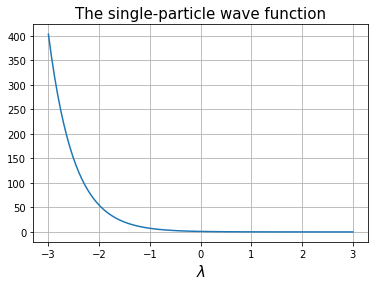
\includegraphics[width=0.6\linewidth]{limits.png}
	\caption{This is a figure of the single-wave function in equation \ref{eq:single_wave}. This figure is used to determine the appropriate integration limits $\lambda$. Here we see that the function is more or less zero for the chosen interval we look at. So we choose the integration limits of the function as $\lambda=1.5$. \label{fig:limits}}
\end{figure}

\begin{table}[htbp]
	\centering
	%\hspace{-1cm}
	\begin{tabular}{ |c|c|c|c|c| }
		\hline \rule{0pt}{13pt}
		Mesh points (N) & Numerical & Analytical & Difference & CPU time [ms]\\
		\hline \rule{0pt}{13pt}
		5 & 0.308692 & 0.192766 & 0.115926 & 1 \\
		\hline \rule{0pt}{13pt}
		10 & 0.154052 & 0.192766 & 0.0387138 & 97 \\
		\hline \rule{0pt}{13pt}
		15 & 0.187130 & 0.192766 & 0.00563558 & 1102 \\
		\hline \rule{0pt}{13pt}
		20 & 0.180469 & 0.192766 & 0.0122967 & 5729 \\
		\hline \rule{0pt}{13pt}
		25 & 0.185593 & 0.192766 & 0.00717284 & 22936 \\
		\hline \rule{0pt}{13pt}
		30 & 0.185011 & 0.192766 & 0.00775459 & 71586 \\
		\hline 
	\end{tabular}	
	\caption{Table for brute force Gaussian-Legendre quadrature integration results with integration limit $\lambda=1.5$. The numerical results are what we get for the given number of mesh points. The differences are means of a number of sets of absolute differences between the numerical and analytical results. The absolute difference decreases and the CPU time, in milliseconds, increases as the mesh points increases. We see that the difference does not decrease all the time as it converges towards zero, but seem to go up and down as the mesh points increases.}
	\label{tab:Gauss_Leg}
\end{table}

\begin{table}[htbp]
	\centering
	%\hspace{-1cm}
	\begin{tabular}{ |c|c|c|c|c| }
		\hline \rule{0pt}{13pt}
		Mesh points (N) & Numerical & Analytical & Difference & CPU time [ms]\\
		\hline \rule{0pt}{13pt}
		5 & 0.174353 & 0.192766 & 0.0184125 & 6 \\
		\hline \rule{0pt}{13pt}
		10 & 0.186544 & 0.192766 & 0.00622209 & 309 \\
		\hline \rule{0pt}{13pt}
		15 & 0.189757 & 0.192766 & 0.00300848 & 4139 \\
		\hline \rule{0pt}{13pt}
		20 & 0.191066 & 0.192766 & 0.00169936 & 23450 \\
		\hline \rule{0pt}{13pt}
		25 & 0.191724 & 0.192766 & 0.00104137 & 96382 \\
		\hline \rule{0pt}{13pt}
		30 & 0.192099 & 0.192766 & 0.000666809 & 354909 \\
		\hline 
	\end{tabular}
	\caption{Table for Gaussian-Laguerre quadrature results for spherical coordinates. For this case we have a more stable and faster decrease in the absolute difference than in Table \ref{tab:Gauss_Leg}. So for the comparison between the numerical and analytical results goes, this improved Gaussian quadrature integration method with Laguerre polynomial and spherical coordinates is better than the brute force with Legendre polynomial. The CPU time, in milliseconds, on the other hand, is a lot higher in this case than for the brute force.}
	\label{tab:Gauss_Lag}
\end{table}

For the brute force Monte Carlo integration method we used the same $\lambda=1.5$ integration limits as for the brute force Gaussian quadrature. In Table \ref{tab:MC_brute} we have the same results as for the Gaussian quadratures, but now we have included the variances. For the Monte Carlo method we have to use mesh points in powers of ten to be able to do the same analysis as before. For this method we get CPU time in microseconds instead of in milliseconds as for the other two methods. So even though the Monte Carlo method needs much higher number of mesh points, the CPU time is much quicker. For lower powers of ten for the mesh points, the numerical results are not as good as for the Gaussian quadratures. As the mesh points get bigger, the numerical results gets better. For around $10^5$ mesh points with CPU time around 56 ms, we reach our goal for third leading digit of the analytical result. If we compare the CPU time for when we reach our goal with the other two methods, we see that the brute force Monte Carlo method is faster even though the number of mesh points are much higher. The variance in the Monte Carlo method is low, but does not change very much as the number of mesh points increase. The CPU time for our chosen number fo mesh points are still well under a second even for one million mesh points.

For the improved Monte Carlo method we changed to spherical methods and used importance sampling. This gave us the results in Table \ref{tab:MC_improved}. As for the brute force Monte Carlo case the improved gave a bad result for low number of mesh points. For the improved we now get faster better results with increasing mesh points. So now we reach our goal within $10^4$ number of mesh points with CPU time around 9 ms. As for the Gaussian quadratures, we now get that the improved method is more accurate for lower number of mesh points than the brute force. Again, the brute force is quicker than the improved if we only look at the same number of mesh points. The variance for the improved Monte Carlo is higher than the brute force for low number of mesh points. For higher mesh points the variance for the improved method decreases much more.

For the final improvement we parallelize the improved Monte Carlo method using openMP and different compiler flags. Since the CPU time is heavily dependent on the background processes of the CPU, the time it takes to run the calculations may very from time to time. That is why we have taken an estimated average of the CPU times to try and find the fastest compiler flag to run with the parallelization. So in Table \ref{tab:MC_opt_compile} we have tested various compiler flags on the improved Monte Carlo method with $10^6$ number of mesh points. There we tested the C++ compiler flags -O1, -O2, -O3 and -Ofast with 4 number of threads for the openMP. From the table we get the best average CPU times for -O3, but -Ofast is not much worse. In Table \ref{tab:MC_parallel} we used compiler flag -O3 for optimal speed-up. Since we have used parallelization on the improved Monte Carlo method, we get almost the same numerical results. The thing that changes the most is the CPU times. From the table we see that the optimal compiler flag and the parallelization makes the calculations a lot faster, especially for higher number of mesh points. For $10^6$ mesh points the calculations now take around 0.4s, while it took around 1s for the improved method and around 0.6s for the brute force. So the parallelization with 4 number of threads and with optimal compiler flag give us the best accuracy of the numerical results and the best CPU time for calculating them.

\begin{table}[htbp]
	\centering
	%\hspace{-1cm}
	\begin{tabular}{ |c|c|c|c|c|c| }
		\hline \rule{0pt}{13pt}
		Mesh points (N) & Numerical & Analytical & Difference & Variance & CPU time [$\mu$s]\\
		\hline \rule{0pt}{13pt}
		$10$ & 0.0520594 & 0.192766 & 0.140706 & $9.60859\cdot10^{-4}$ & 3 \\
		\hline \rule{0pt}{13pt}
		$10^2$ & 0.0858179 & 0.192766 & 0.106948 & $2.56645\cdot10^{-3}$ & 5 \\
		\hline \rule{0pt}{13pt}
		$10^3$ & 0.108695 & 0.192766 & 0.0840702 & $4.91805\cdot10^{-4}$ & 964 \\
		\hline \rule{0pt}{13pt}
		$10^4$ & 0.160121 & 0.192766 & 0.0326449 & $3.90958\cdot10^{-4}$ & 6283 \\
		\hline \rule{0pt}{13pt}
		$10^5$ & 0.196523 & 0.192766 & 0.00375685 & $1.15132\cdot10^{-4}$ & 55835 \\
		\hline \rule{0pt}{13pt}
		$10^6$ & 0.193233 & 0.192766 & 0.000467207 & $1.99508\cdot10^{-5}$ & 573519 \\
		\hline 
	\end{tabular}	
	\caption{Table for brute force Monte Carlo integration results with integration limit $\lambda=1.5$. For this method we see that for mesh points up to around $10^4$, the numerical results are worse than for the Gaussian quadrature methods. With higher mesh points than this, the numerical results become very good. The CPU time, in microseconds, for this brute force Monte Carlo, is much better than for the Gaussian quadratures. For around N=30 the CPU time were in seconds for Gaussian quadrature, but for this Monte Carlo method we use around half a second for N=$10^6$. The variance is low, and decreases a little as the mesh points increases.}
	\label{tab:MC_brute}
\end{table}

\begin{table}[htbp]
	\centering
	%\hspace{-1cm}
	\begin{tabular}{ |c|c|c|c|c|c| }
		\hline \rule{0pt}{13pt}
		Mesh points (N) & Numerical & Analytical & Error & Variance & CPU time [$\mu$s]\\
		\hline \rule{0pt}{13pt}
		$10$ & 0.365879 & 0.192766 & 0.173114 & $4.59202\cdot10^{-2}$ & 0 \\
		\hline \rule{0pt}{13pt}
		$10^2$ & 0.155251 & 0.192766 & 0.0375148 & $1.56870\cdot10^{-3}$ & 47 \\
		\hline \rule{0pt}{13pt}
		$10^3$ & 0.173329 & 0.192766 & 0.0194369 & $2.87435\cdot10^{-4}$ & 1258 \\
		\hline \rule{0pt}{13pt}
		$10^4$ & 0.188290 & 0.192766 & 0.00447596 & $9.22912\cdot10^{-5}$ & 9294 \\
		\hline \rule{0pt}{13pt}
		$10^5$ & 0.187134 & 0.192766 & 0.00563153 & $8.96394\cdot10^{-6}$ & 105771 \\
		\hline \rule{0pt}{13pt}
		$10^6$ & 0.191672 & 0.192766 & 0.00109395 & $9.26449\cdot10^{-7}$ & 994728 \\
		\hline 
	\end{tabular}	
	\caption{Table for improved Monte Carlo integration results for spherical coordinates. This improved Monte Carlo method gives a better absolute difference between the numerical and analytical results for lower number of mesh points than the brute force Monte Carlo in Table \ref{tab:MC_brute}. Fo higher mesh points, it seems like the brute force is a little more accurate. As in the Gaussian quadrature cases, the improved method with spherical coordinates seem to use longer CPU time than the brute forces. For the Monte Carlo methods, the time increase between the methods is not that high and are still in microseconds. The variance for the improved Monte Carlo is higher for for lower mesh points, but decreases more as the mesh points increases. For N=$10^{6}$ mesh points the variance in the improved method is much lower than for the brute force.}
	\label{tab:MC_improved}
\end{table}

\begin{table}[htbp]
	\centering
	%\hspace{-1cm}
	\begin{tabular}{ |c|c|c|c|c| }
		\hline \rule{0pt}{13pt}
		Compiler flags & -O1 & -O2 & -O3 & -Ofast \\
		\hline \rule{0pt}{13pt}
		CPU time [$\mu$s] & 597584 & 521989 & 439243 & 446278 \\
		\hline 
	\end{tabular}	
	\caption{Table for parallelized Monte Carlo integration results for 8 number of threads and $N=10^6$ number of mesh points. Comparing the CPU time for different C++ compiler flags. Here we see that -O3 seems to be the fastest in our case.}
	\label{tab:MC_opt_compile}
\end{table}

\begin{table}[htbp]
	\centering
	%\hspace{-1cm}
	\begin{tabular}{ |c|c|c|c|c|c| }
	\hline \rule{0pt}{13pt}
	Mesh points (N) & Numerical & Analytical & Error & Variance & CPU time [$\mu$s]\\
	\hline \rule{0pt}{13pt}
	$10$ & 0.0279664 & 0.192766 & 0.164799 & $3.45445\cdot10^{-4}$ & 0 \\
	\hline \rule{0pt}{13pt}
	$10^2$ & 0.172129 & 0.192766 & 0.0206368 & $3.46750\cdot10^{-3}$ & 8 \\
	\hline \rule{0pt}{13pt}
	$10^3$ & 0.203862 & 0.192766 & 0.0110960 & $6.54114\cdot10^{-4}$ & 998 \\
	\hline \rule{0pt}{13pt}
	$10^4$ & 0.200041 & 0.192766 & 0.00727570 & $1.03580\cdot10^{-4}$ & 4823 \\
	\hline \rule{0pt}{13pt}
	$10^5$ & 0.191634 & 0.192766 & 0.00113139 & $7.91637\cdot10^{-6}$ & 42656 \\
	\hline \rule{0pt}{13pt}
	$10^6$ & 0.193930 & 0.192766 & 0.00116442 & $9.97261\cdot10^{-7}$ & 418861 \\
	\hline 
\end{tabular}	
	\caption{Table for parallelized Monte Carlo integration results for spherical coordinates and with 4 number of threads. This is run with the compiler flag \textbf{-O3} in C++, since this gave the best CPU times (as seen in Table \ref{tab:MC_opt_compile}). The results we get are close to the ones in Table \ref{tab:MC_improved} for the improved Monte Carlo, except that in this case the CPU time, in microseconds, is much better. This is exactly what we wanted with the parallelization. For chosen higher number of threads than what we have chosen, the CPU time decreases but then the numerical results are get worse. For lower number of threads the numerical results are closer to the analytical, but has higher CPU time. So the chosen 4 number of threads is a compromise between the accuracy and CPU time.}
	\label{tab:MC_parallel}
\end{table}

When running the C++ program directly in QT Creator we get different results and CPU times then if we run the program in a terminal window. This happens especially for the Monte Carlo methods. In the terminal window we get the same results for the improved and parallelized Monte Carlo, and only the CPU times change. There, changing the number of threads does not seem to change anything. When we run the program directly in QT Creator, then the results and CPU times change when changing the number of threads for openMP. That is why we choose 4 number of threads, since this seem to give a good compromise between the numerical results and the CPU time. For lower number of threads we get better numerical results, but longer CPU time. For higher number of threads we get better CPU time, but worse numerical results.

\section{Conclusion}
For this project we wanted to test various numerical integration methods to see which method is best, and how our results changes for more brute force methods versus more improved and thought out methods. We have used brute force Gaussian-Legendre quadrature, improved Gaussian quadrature with Laguerre polynomial and spherical coordinates, brute force Monte Carlo integration with uniform distribution, improved Monte Carlo integration with importance sampling, exponential distribution and spherical coordinates and lastly parallelized Monte Carlo integration with openMP and compiler flags.

We have studied the differences in the methods by looking at the difference in the numerical and analytical results, variances and CPU times with increasing number of mesh points. From these results we have come to the conclusion that the parallelized Monte Carlo is the best method in both accuracy to the analytic answer and the CPU time of the calculations for high number of mesh points. This seems to be as expected since Monte Carlo is expected to work best for multidimensional cases, like our case here where we look at a six-dimensional integral. For both the Gaussian quadrature and Monte Carlo the improved methods are more accurate than the brute force, but the brute force methods seem to be faster for the same number of mesh points. 

For the integral we had to work the possibility of dividing by zero. So to avoid that, we just said that the whole function got the value zero when $|\textbf{r}_1-\textbf{r}_2|=0$. An improvement in the future could be to rewrite the integral to avoid this kind of trouble with dividing by zero. We have also excluded a normalization factor in the final integral in equation \ref{eq:integral} that we solved. Future work could be to include this normalization factor in the calculations.

\appendix
\section{Appendix}
\label{sect:appendix}
Link to GitHub repository:\\
\end{document}
